\documentclass[main]{subfiles}
\begin{document}
\chapter{座標変換したセンサデータをプロットする}

これは講義資料「第4回 オドメトリと座標系」内の課題です。

\section{課題概要}
測域センサをつけたフリー状態(外力を受けて動く状態)の
ロボットを動かしてマッピングする。

ロボットを中心とした「方向」と「距離」の情報をもつ
極座標系のデータをセンサから受け取り、
ロボットを原点(0, 0)\footnote{(X座標, Y座標)}
とする直交座標系のデータ(FS座標系データ)に変換するだけの
プログラムが与えられる。
これをスタート地点を原点(0, 0)とする平面に関して唯一の値をとる
直交座標系のデータ(GL座標系データ)に変換する処理を記述してマッピングを行う。

\section{測域センサの概要}
測域センサには北陽電機株式会社のURG-04LXを使用する。
ロボットの前方に取り付けられたセンサはPCとUSB接続され、
PCとの通信にはSCIP2.0という通信プロトコルを利用する。

\section{解法}
\begin{figure}[H]
	\begin{minipage}{0.5\hsize}
		\setlength{\parindent}{1\Cwd}
		FS座標系もGL座標系も同一平面上の点の位置を定めるものなので、
		FS座標系で表現される点をGL座標系に変換するには、
		\textbf{現在地のGL座標}とスタート地点において$\theta = 0$と定義する
		\textbf{ロボットの傾き$\theta$}(rad)が必要となる。

		具体的な処理を明確にするためにプログラムを設計する前に右のような図を描いた。
		目的は、FS座標(Px, Py)で表現される赤い点をGL座標(glPx, glPy)に変換することだ。
		図ではXやYの表示が逆転しているものもあるが、軸に関しては正しく表示しているので
		パラメータの仮変数だと思って無視していただきたい。
	\end{minipage}
	\begin{minipage}{0.5\hsize}
		\begin{figure}[H]
			\centering
			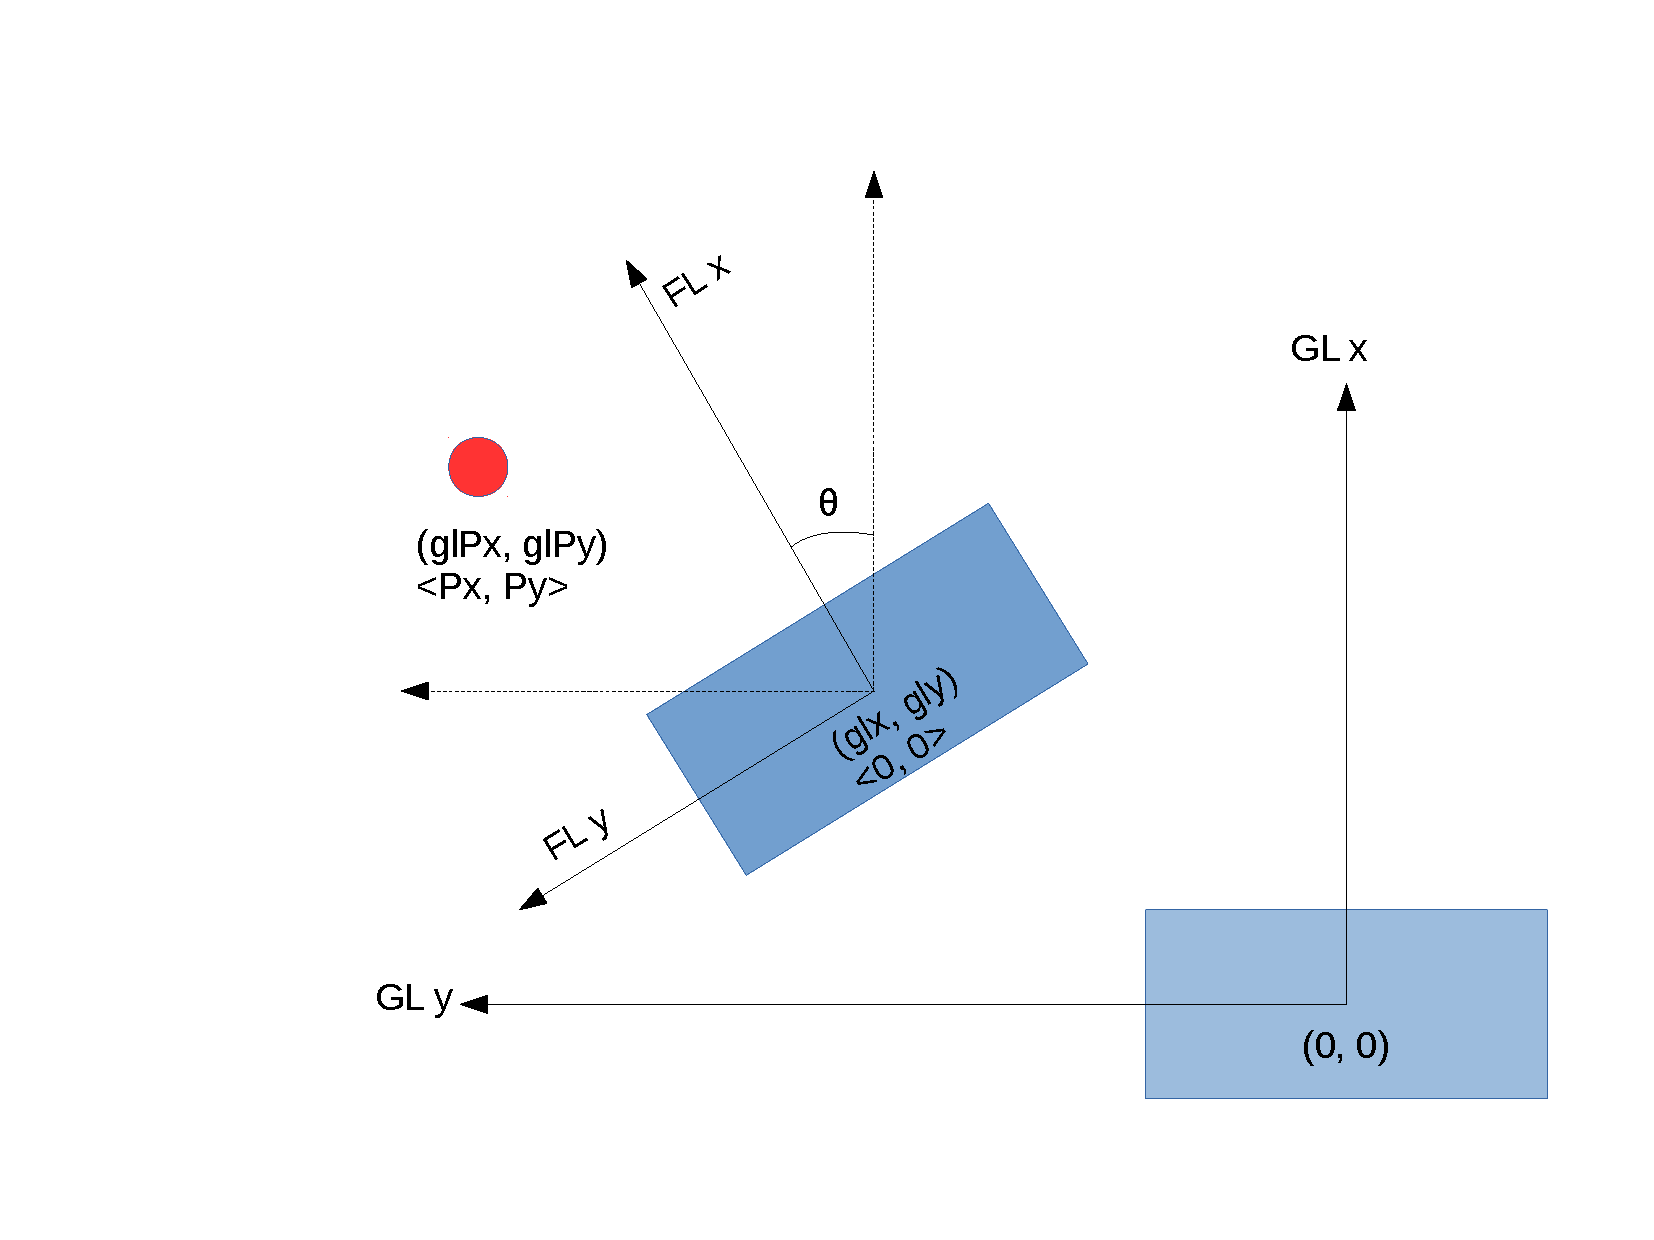
\includegraphics[width=8cm]{./trans.pdf}
			\caption{FS座標系とGL座標系の関係}
		\end{figure}
	\end{minipage}
\end{figure}
% まず現在のロボットの傾き\textit{pos\_theta\_gl}を利用して座標を回転させる。
% 座標の回転といっても同一平面の点の回転移動と同じであるから、
% 以下のような行列計算で求めることができる。
% 幾何的に考え。
% 最後に現在地のGL座標(pos\_x\_gl, pos\_y\_gl)を取得したFS座標に加算することで平行移動
% これはFS座標における点へのベクトルとGL座標におけるロボット中心へのベクトルの加算
% を行うものであり、

\section{結果}
ノイズの多さが目立つが正しくマッピングできている。

\section{考察}

\end{document}
